\documentclass[a4paper]{article}

\usepackage[T1]{fontenc}
\usepackage[utf8]{inputenc}
\usepackage[english]{babel}
\usepackage{csquotes}
\usepackage{listings}
\usepackage{multicol}
\lstset{language=c,frame=single,captionpos=b}
\usepackage{hyperref}
\usepackage{amsmath}
\usepackage[backend=biber, sorting=none,maxbibnames=40]{biblatex}
\renewbibmacro{in:}{}
\addbibresource{ref.bib}
\usepackage{graphicx}
\usepackage{placeins}
\usepackage[margin=2.5cm]{geometry}
\usepackage{subcaption}
\usepackage[affil-it]{authblk}
\usepackage{color}
\usepackage{amssymb,amsmath}
\usepackage{subfloat}
\usepackage{float}

\begin{document}
\title{GPU Assignment: Image processing}
\author{Stefano Sandonà}
\affil{Vrije Universiteit Amsterdam, Holland}
\date{}
		
\maketitle

\section{GPUs: NVIDIA GTX480}
\label{sec:nvidia}
The aim of this assignment was to learn how to use many-core accelerators, GPUs in this particular case, to parallelize data-intensive code. All the implementations were written for the \textbf{NVIDIA GTX480}, using CUDA, a parallel computing platform and programming model invented by NVIDIA. Programming with CUDA, there is a straightforward mapping onto hardware, for this reason it is necessary to study the available HW before start developing an application. The architecture of the given accelerator is is shown in Figure \ref{fig:gtx}, its main characteristics and limits are shown in Table \ref{table:t1}.

\begin{figure}[ht]
    \centering
    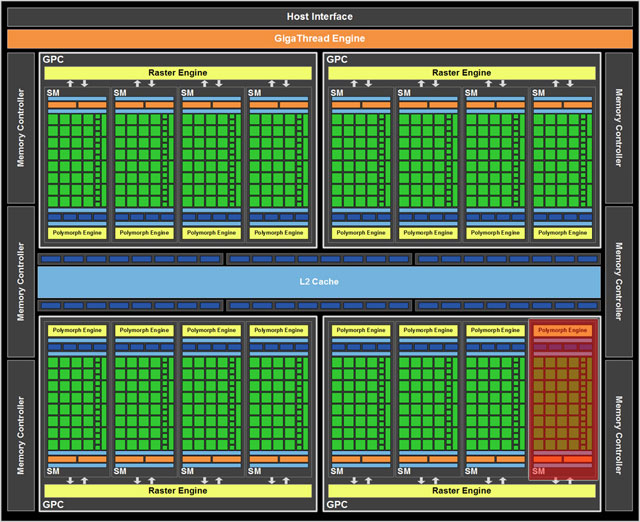
\includegraphics[width=0.7\linewidth]{gtx}
    \caption{NVIDIA GTX480 Architecture}
    \label{fig:gtx}
\end{figure}
\FloatBarrier

\begin{table}[ht]
\centering
\begin{tabular}{l|l}
Microarchitecture & Fermi \\ \hline
Compute capability (version) & 2.0 \\ \hline
Maximum dimensionality of grid of thread blocks & 3 \\ \hline
Maximum x-dimension of a grid of thread blocks & 65535 \\ \hline
Maximum y-, or z-dimension of a grid of thread blocks & 65535 \\ \hline
Maximum dimensionality of thread block & 3 \\ \hline
Maximum x- or y-dimension of a block & 1024 \\ \hline
Maximum number of threads per block & 1024 \\ \hline
Cores per SM (warp size) & 32 \\ \hline
SM & 15 \\ \hline
Cores & 480 (32 * 15) \\ \hline
Maximum number of resident blocks per multiprocessor & 8 \\ \hline
Maximum number of resident warps per multiprocessor & 48 \\ \hline
Maximum number of resident threads per multiprocessor & 1536 (48 * 32) \\ \hline
Number of 32-bit registers per multiprocessor & 32K \\ \hline
Maximum amount of shared memory per multiprocessor & 48K
\end{tabular}
\caption{NVIDIA GTX480 Specifications}
\label{table:t1}
\end{table}


\section{CImg}
\label{sec:cimg}
The image processing library used in this project was CImg, a small, modern and open-source toolkit developed for C++. CImg implements the RGB color model, an additive color model in which red, green, and blue light are added together in various ways to reproduce a broad array of colors. Each colored image of size \textit{N*M} is composed by three parts (R,G,B) of the same size, so that \textit{N*M*3} values are necessary to define an image. The Figure \ref{fig:rgb} shows an example of image composition.

\begin{figure}[ht]
    \centering
    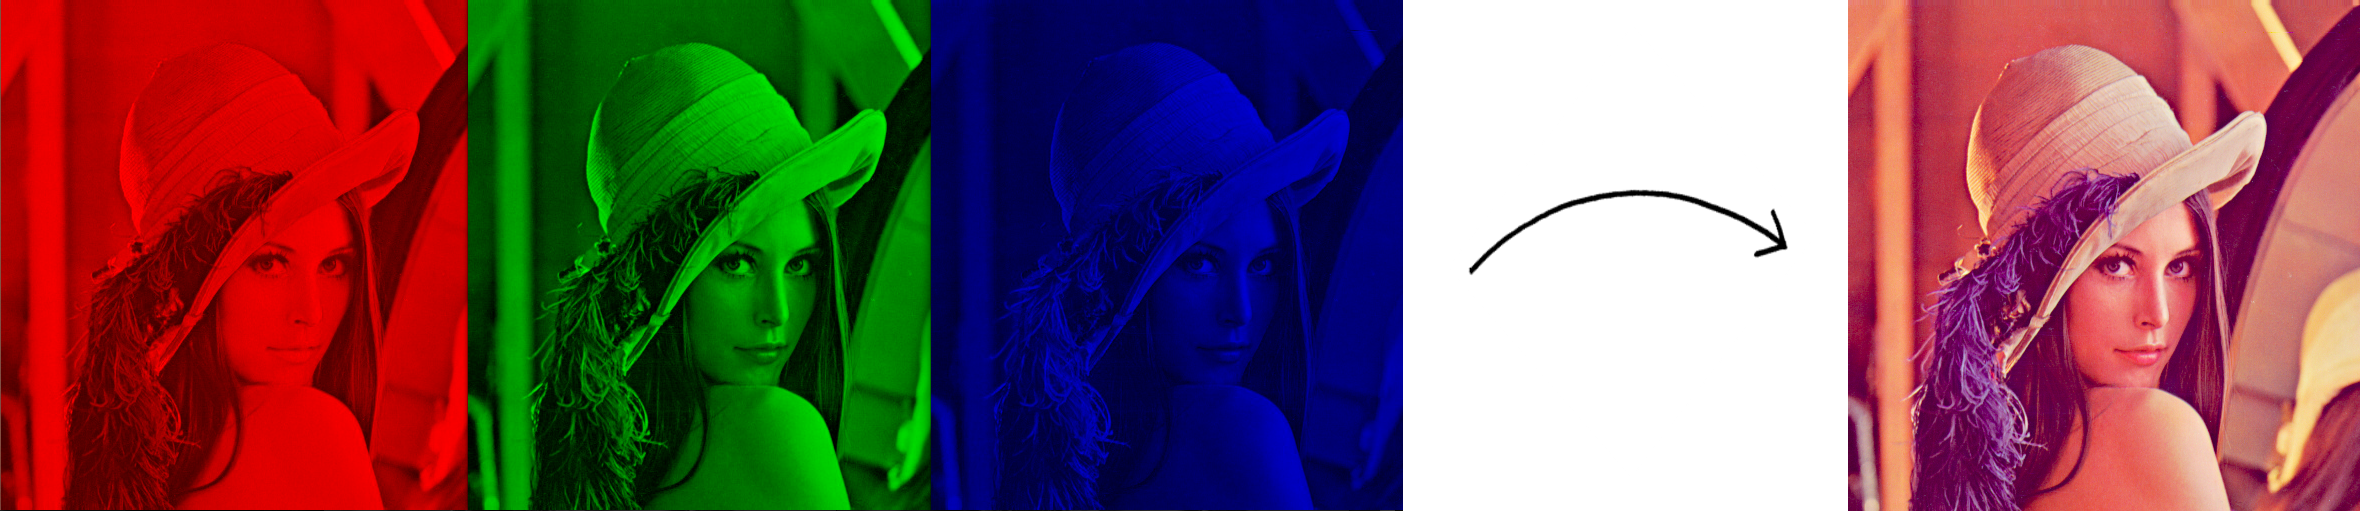
\includegraphics[width=0.7\linewidth]{rgb}
    \caption{RGB model}
    \label{fig:rgb}
\end{figure}
\FloatBarrier

\section{The processing flow}
\label{sec:cpf}
Using CUDA there are two parts of the code: the device code, or GPU code, or the Kernel, that is a sequential program, write for one thread and execute for all and the HOST code, or CPU code, that is used to instantiate the grid, run the kernel, manage the memory. Figure \ref{fig:flow} shows the processing flow of a CUDA application. In the particular case of image processig, everything starts from the CPU, that store the image from a file into a local buffer, allocates IN and OUT buffers on the GPU (\textit{cudaMalloc}) and copy the image into the GPU's IN buffer (\textit{cudaMemCpy}). After that, the CPU launches the GPU kernel with a defined grid configuration (\textit{kernel\_function <<gridDim, blockDim>>(params)}), that is executed by the GPU following the SIMT (Single Instruction, Multiple Threads) NVIDIA model. The threads are executed in parallel in each core, and they read the assigned part of IN data and generates the assigned part of OUT data. At the end, the results are copied out back to the CPU (\textit{cudaMemCpy}) and the image is written to a file by the CPU.

\begin{figure}[ht]
    \centering
    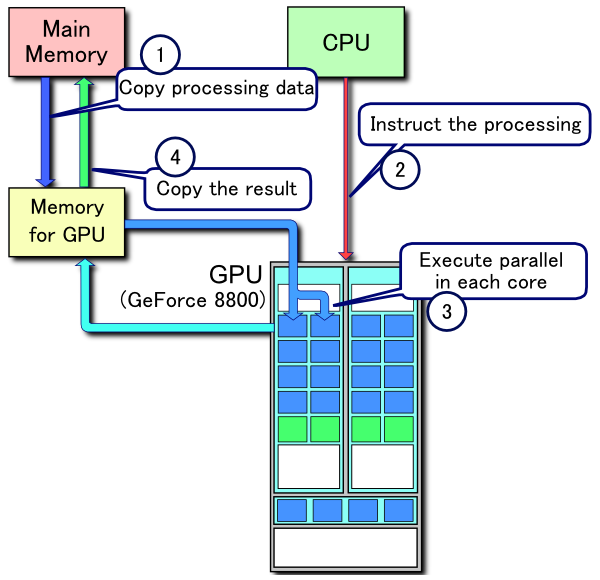
\includegraphics[width=0.5\linewidth]{flow}
    \caption{CUDA processing flow}
    \label{fig:flow}
\end{figure}
\FloatBarrier

\section{CUDA grid configuration}
\label{sec:grid}
In CUDA, as mentioned before, there is a strinct mapping with the hardware, so that an hardware virtualization model is fixed with the concepts of thread, block and grid.
Each \textbf{thread} executes the kernel code, running on one CUDA core.
The threads are logically grouped into \textbf{thread blocks}, so that the threads of the same block will run on the same multiprocessor. The thread blocks are logically organized in a \textbf{Grid}, that represent the entire dataset. The blocks and the grid can be of 1D, 2D or 3D.
An image is a 2D structure and for this reason the most convenient choice is to set up also a 2D grid. However, setting up a 2D grid, there is not only one way to follow. For this particular project, 4 possible combinations were considered. The first was a non square grid of 1D blocks (Figure \ref{fig:ns1}), the second a square grid with 1D blocks (Figure \ref{fig:s1}), the third a non square grid of 2D blocks (Figure \ref{fig:ns2}) and the third a square grid of 2D blocks (Figure \ref{fig:s2}). Different configurations were tested in order to find the best to suit the particular case.

\begin{figure}[!ht]
\begin{subfigure}{0.5\textwidth}
\centering
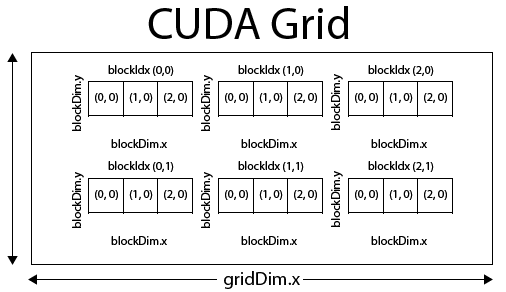
\includegraphics[width=\linewidth]{res/1D_no_square}
\caption{No square grid with 1D blocks}
\label{fig:ns1}
\end{subfigure} % separation between the subfigures
\begin{subfigure}{0.5\textwidth}
\centering
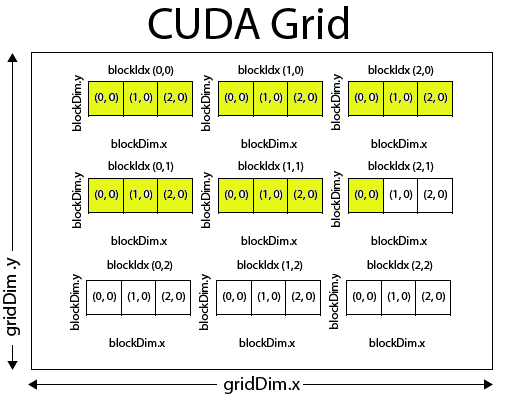
\includegraphics[width=\linewidth]{res/1D_square}
\caption{Square grid with 1D blocks}
\label{fig:s1}
\end{subfigure}
 % separation between the subfigures
\begin{subfigure}{0.5\textwidth}
\centering
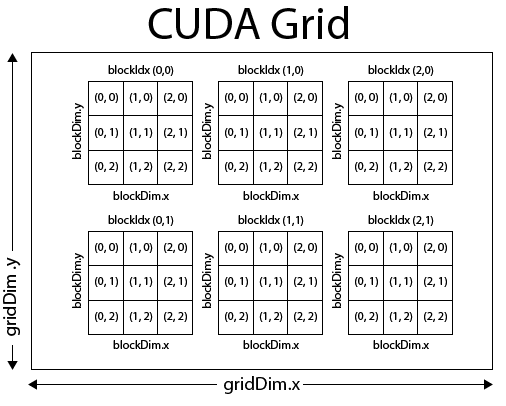
\includegraphics[width=\linewidth]{res/2D_no_square}
\caption{No square grid with 2D blocks}
\label{fig:ns2}
\end{subfigure}
 % separation between the subfigures
\begin{subfigure}{0.5\textwidth}
\centering
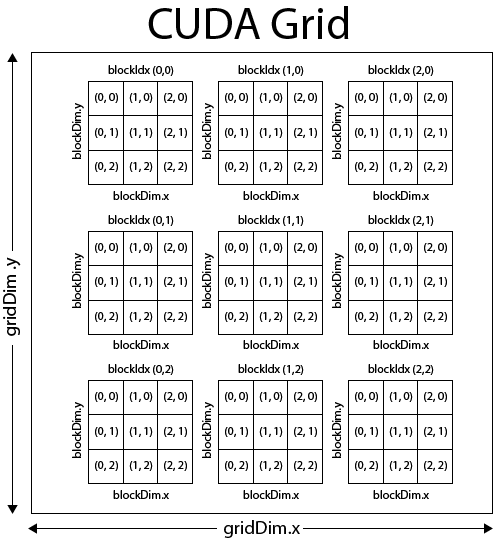
\includegraphics[width=\linewidth]{res/2D_square}
\caption{Square grid with 2D blocks}
\label{fig:s2}
\end{subfigure}
\caption{Possible kernel configurations}
 \label{fig:speed}
\end{figure}
\FloatBarrier

\section{Coalesced memory access}
\label{sec:cma}
One of the main bottlenecks with the GPUs is the global memory access that is expensive. CUDA uses a SIMT approach, in which all threads of a warp execute the same instruction. If the kernel is correctly designed, when the threads of a warp ask a value stored in the global memory, instead of have one access per thread, these accesses can be grouped if consecutive threads access consecutive memory addresses. This practise, is very useful to reduce the memory overhead, so that it was adopted in each algorithm.


\section{Algorithm 1: Grayscale Conversion and Darkening}
\label{sec:gcd}
From an RGB image, the output of this algorithm is a darker grayscale image.
The gray value of a pixel is generated by weighting the three values (\texttt{0.3*R, 0.59*G, 0.11*B}) and then summing them together. To darken the obtained grayscale image, the final pixel value is multiplied by a constant (0.6). The Figure \ref{fig:dark} shows an example of the result. The sequential algorithm, simply go through the entire image and computes for each pixel the corresponding value.

\begin{figure}[ht]
    \centering
    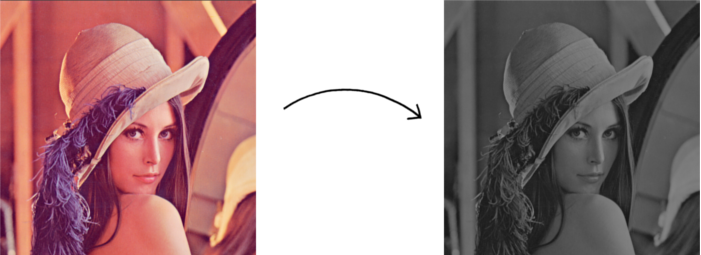
\includegraphics[width=\linewidth]{dark}
    \caption{Grayscale Conversion and Darkening}
    \label{fig:dark}
\end{figure}
\FloatBarrier

\subsection{Parallelization}
\label{sec:p1}
\subsection{First method}
\label{sec:fm}
The first attempt was done to understand the best grid configuration. To exploit the coalesced memory access, two consecutive threads computes/accesses the values of two consecutive pixels.




\begin{figure}[ht]
    \centering
    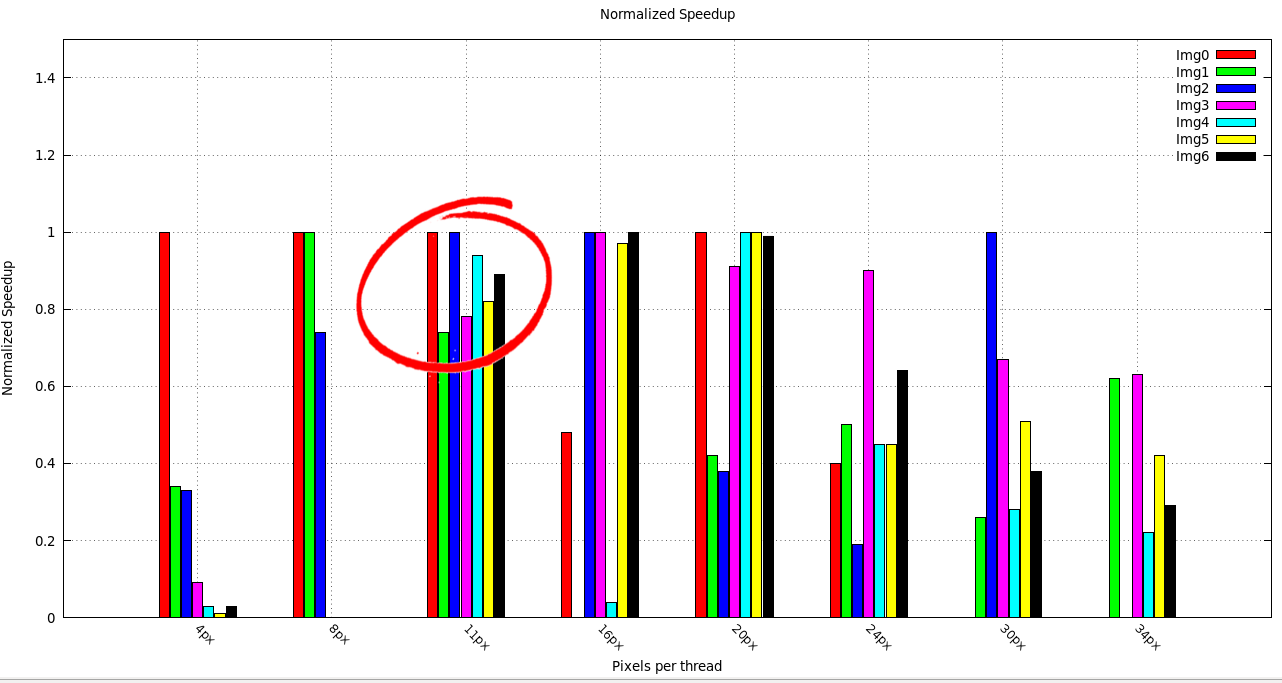
\includegraphics[width=0.9\linewidth]{res/histogram_darker}
    \caption{Normalized Speedup}
    \label{fig:norm_histo_darker}
\end{figure}
\FloatBarrier

\section{Algorithm 2: Histogram Computation}
\label{sec:hc}
From an RGB image, the output of this algorithm is a grayscale image with the relative histogram of 256 possible values of gray.
The histogram measures how often a value of gray is used in an image. The sequential algorithm, simply go through the entire image, computing for each pixel the corresponding gray value and incrementing the corresponding counter. The Figure \ref{fig:histo} shows an example of the result.

\begin{figure}[ht]
    \centering
    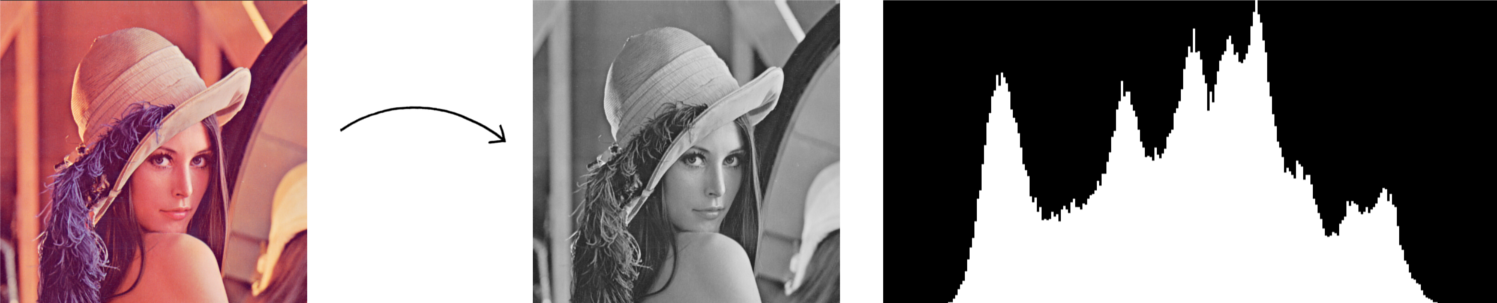
\includegraphics[width=0.7\linewidth]{histo}
    \caption{Histogram Computation}
    \label{fig:histo}
\end{figure}
\FloatBarrier

\section{Algorithm 3: Smoothing}
\label{sec:smoo}
Smoothing is the process of removing noise from an image by the means of statistical analysis. To remove the noise, each point is replaced by a weighted average of its neighbours. In this way small-scale structures are removed from the image. In this case a two-dimensional 5-point triangular smooth filter was used. The Figure \ref{fig:smooth} shows an example of the result.

\begin{figure}[ht]
    \centering
    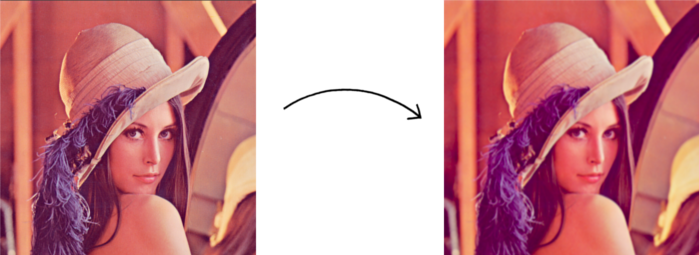
\includegraphics[width=0.5\linewidth]{smooth}
    \caption{Smoothing}
    \label{fig:smooth}
\end{figure}
\FloatBarrier


\printbibliography 

\end{document}

			 	 